\documentclass[11pt,a4paper]{article}
\usepackage[T1]{fontenc}
\usepackage[utf8]{inputenc}
\usepackage[french]{babel}
\usepackage{geometry}
\usepackage{graphicx}
\usepackage{booktabs}
\usepackage{listings}
\usepackage{hyperref}
\usepackage{float}
\usepackage{longtable}

\geometry{margin=2.2cm}
\setlength{\emergencystretch}{2em}
\hypersetup{colorlinks=true,linkcolor=blue,urlcolor=blue}
\lstset{basicstyle=\ttfamily\small,breaklines=true,frame=single,language=C++}

\title{Rapport technique, Lab 5\\
\large Boucle fermée sur la livraison mesurée\\
Dépôt \texttt{ns3\_IMT2030\_connectivity}}
\author{Traorehub, travail de recherche en cours}
\date{Novembre 2026}

\begin{document}
\maketitle
\tableofcontents
\newpage

\section{Objectif}

Le Lab 3 a montré qu'un plafond fixe élève le taux de livraison des octets émis et diminue le volume reçu. Le canal redevient disponible dès que les stations admises ont épuisé leur budget de 40 paquets, et les stations exclues ne l'utilisent jamais. Le Lab 5 demande si une boucle qui observe la livraison récente peut réadmettre des stations à temps pour augmenter ce volume.

La boucle n'est pas un modèle entraîné. Elle n'utilise pas \texttt{ns3-gym}. Elle applique deux seuils à une mesure, puis elle élargit ou réduit le plafond. Elle tient le rôle d'une boucle métrique, décision, action, qui est le pas prévu avant un contrôleur appris. La radio reste le proxy Wi-Fi 802.11n, avec Yans, \texttt{HtMcs7} et le SSID \texttt{imt2030-dense-zone}. Le module NR étant absent, aucun chiffre de ce rapport n'est un résultat 5G.

\section{Loi}

Le plafond initial est celui du Lab 3, avec une capacité de référence de 3~Mbit/s. Toutes les 0,5~s, le contrôleur compare les octets arrivés pendant la fenêtre aux octets réellement émis pendant la même fenêtre. Si ce rapport est inférieur à 0,35, le plafond baisse d'au moins un terminal, et d'environ un sixième de sa valeur. S'il est supérieur à 0,50, le plafond monte d'au moins un terminal, et d'environ un douzième de sa valeur. Entre les deux seuils, le plafond ne change pas. L'admission continue de suivre l'indice de grille. Elle ne classe pas les terminaux par qualité radio.

\begin{lstlisting}
if (ratio < 0.35 && cap > 1)
    cap -= max(1, cap / 6);
else if (ratio > 0.50 && cap < nSta)
    cap += max(1, cap / 12);
\end{lstlisting}

Les politiques \texttt{baseline} et \texttt{adaptive} du binaire n'ont pas été modifiées. Une sonde sur 100 terminaux et 40~ms en mode \texttt{adaptive} a retrouvé les 287\,744 octets, le taux 0,585, les 76 événements et les 24 flux du Lab 3. La comparaison ci-dessous rapproche donc la nouvelle politique des CSV déjà publiés, sur le même émetteur.

\section{Protocole}

Douze runs couvrent \texttt{gridSide} dans $\{4, 6, 8, 10\}$ et \texttt{intervalMs} dans $\{40, 80, 160\}$, pour la seule politique \texttt{feedback}. La durée vaut 10~s. Le budget reste de 40 paquets de 512 octets. L'animation est désactivée. Une seule graine est utilisée. Le CSV est \texttt{resultats.csv} dans les sorties du Lab 5. La colonne \texttt{finalCap} donne le plafond à la fin du run. Elle ne donne pas le nombre de stations émettrices à chaque instant.

\section{Résultats de la boucle}

\begin{longtable}{@{}rrrrrrrr@{}}
\caption{Politique feedback, durée 10~s, capacité de référence 3~Mbit/s.}\\
\toprule
STA & ms & Livraison & Jain & Throttle & Octets reçus & Flux & Plafond \\
\midrule
\endfirsthead
\toprule
STA & ms & Livraison & Jain & Throttle & Octets reçus & Flux & Plafond \\
\midrule
\endhead
16 & 40 & 1,000 & 1,000 & 4 & 327\,680 & 16 & 16 \\
16 & 80 & 1,000 & 1,000 & 4 & 327\,680 & 16 & 16 \\
16 & 160 & 1,000 & 1,000 & 4 & 327\,680 & 16 & 16 \\
36 & 40 & 0,969 & 0,994 & 32 & 714\,752 & 36 & 36 \\
36 & 80 & 0,966 & 0,995 & 12 & 712\,192 & 36 & 36 \\
36 & 160 & 0,981 & 0,998 & 12 & 723\,456 & 36 & 36 \\
64 & 40 & 0,829 & 0,964 & 84 & 854\,016 & 52 & 44 \\
64 & 80 & 0,677 & 0,939 & 63 & 745\,472 & 61 & 43 \\
64 & 160 & 0,656 & 0,981 & 57 & 815\,616 & 64 & 45 \\
100 & 40 & 0,819 & 0,889 & 116 & 865\,280 & 56 & 56 \\
100 & 80 & 0,552 & 0,855 & 101 & 718\,336 & 65 & 65 \\
100 & 160 & 0,521 & 0,857 & 134 & 783\,360 & 91 & 54 \\
\bottomrule
\end{longtable}

\begin{figure}[H]
  \centering
  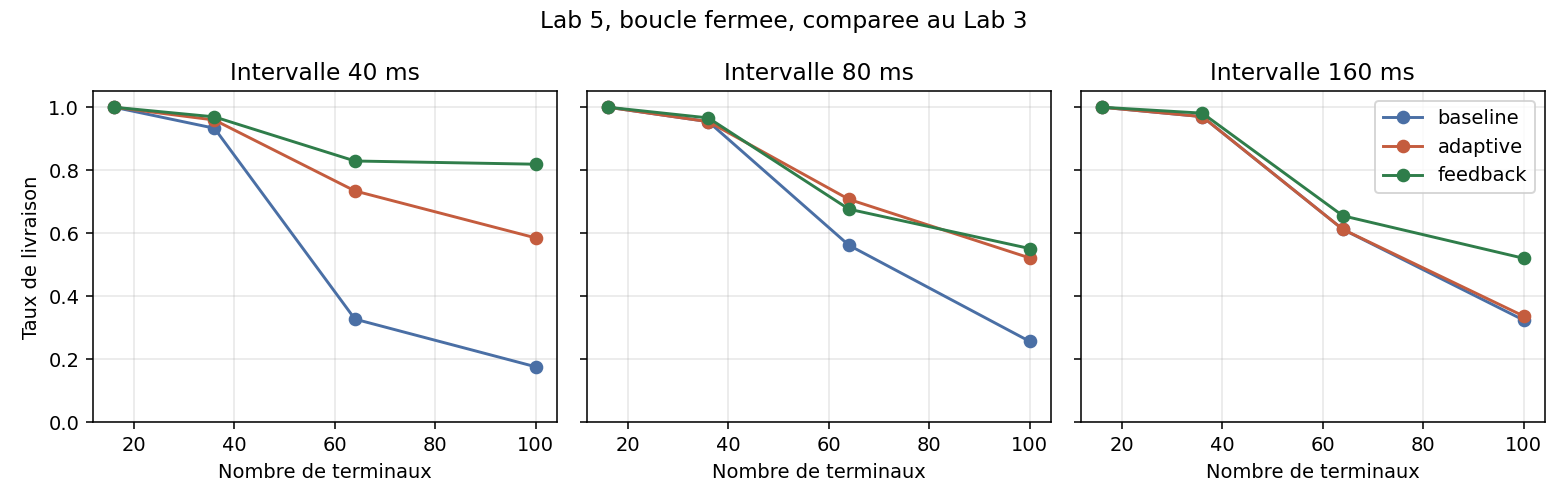
\includegraphics[width=\linewidth]{../../labs/lab05_ai_native/sorties/livraison_campagne.png}
  \caption{Taux de livraison des octets émis. La courbe feedback est rapprochée des politiques baseline et adaptive du Lab 3, produites avec le même émetteur.}
\end{figure}

\begin{figure}[H]
  \centering
  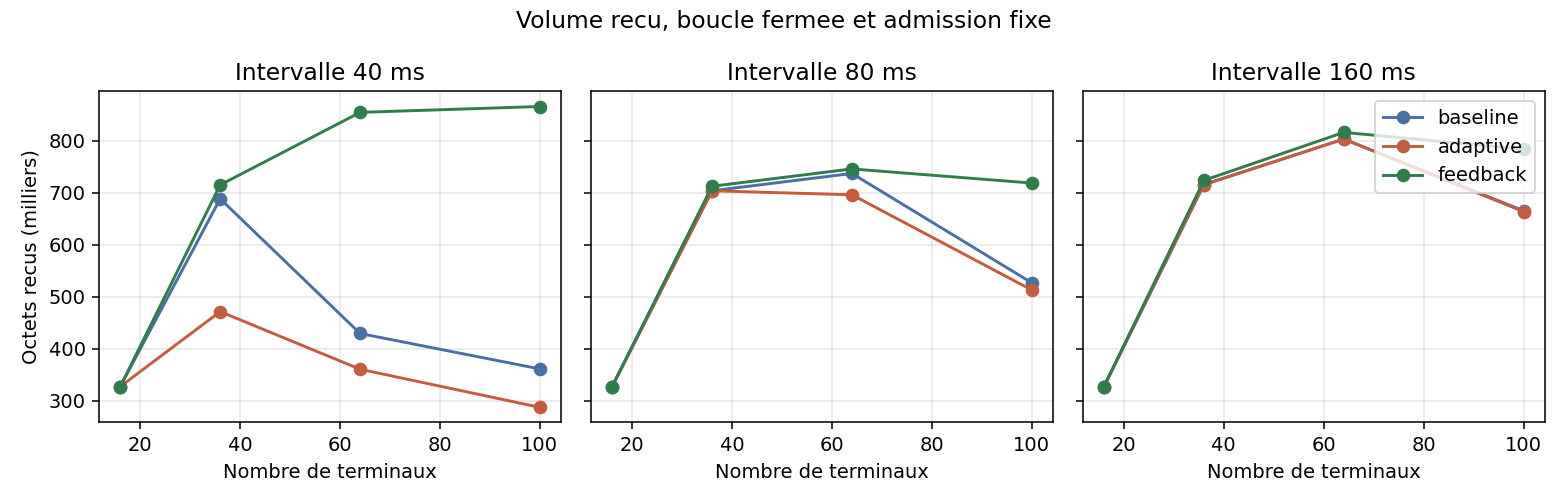
\includegraphics[width=\linewidth]{../../labs/lab05_ai_native/sorties/octets_campagne.png}
  \caption{Octets reçus par le point d'accès. Sur les cellules chargées, la boucle fermée dépasse à la fois l'émission simultanée et l'admission fixe.}
\end{figure}

\section{Lecture par régime}

Sur 16 terminaux, le volume reste 327\,680 octets et le taux reste 1, comme en baseline. Quatre événements apparaissent. Ils correspondent à un mouvement transitoire du plafond, qui revient à 16. Le service final n'en est pas modifié. Tous les paquets prévus arrivent.

Sur 36 terminaux, la boucle termine avec les 36 stations admises. À 40~ms, elle reçoit 714\,752 octets, contre 688\,128 en baseline et 471\,552 avec le plafond fixe de 24. Le taux vaut 0,969, contre 0,933 et 0,959. À 80~ms et à 160~ms, le gain de volume est plus faible, de l'ordre de quelques milliers d'octets. Une seule graine ne permet pas de traiter ces petits écarts comme un effet stabilisé. La direction, en revanche, est la même.

Sur 64 terminaux à 40~ms, l'écart devient large. La baseline reçoit 429\,568 octets, avec un taux de 0,328. L'admission fixe reçoit 360\,960 octets, avec un taux de 0,734. La boucle reçoit 854\,016 octets, avec un taux de 0,829, 52 flux et un plafond final de 44. Le volume dépasse les deux références, et le taux aussi. À 80~ms, le volume de la boucle, 745\,472 octets, dépasse la baseline, 736\,768, et l'admission fixe, 695\,808. Le taux, 0,677, reste au-dessus de la baseline, 0,562, et passe sous le taux de l'admission fixe, 0,708. Cette cellule empêche de dire que la boucle domine les deux métriques partout. Elle domine le volume sur cette cellule, et elle cède un peu de taux à l'admission fixe. À 160~ms, le volume passe de 802\,816 à 815\,616 octets et le taux de 0,613 à 0,656.

Sur 100 terminaux, les trois intervalles vont dans le même sens. À 40~ms, la baseline livre 706 paquets sur 4\,000, soit 361\,472 octets et un taux de 0,177. L'admission fixe livre 562 paquets sur 960, soit 287\,744 octets et un taux de 0,585. La boucle livre 1\,690 paquets sur 2\,063 émis, soit 865\,280 octets et un taux de 0,819, avec 56 flux et un plafond final de 56. Le volume est environ 2,4 fois celui de la baseline et environ 3,0 fois celui de l'admission fixe. À 80~ms, la boucle reçoit 718\,336 octets, contre 526\,848 et 513\,024. À 160~ms, elle reçoit 783\,360 octets, contre 665\,088 et 663\,552, avec un taux de 0,521 contre 0,325 et 0,338.

\section{Mécanisme compatible avec le budget fini}

Chaque station s'arrête après 40 paquets, qu'elle soit encore admise ou non. À 40~ms, ces 40 paquets occupent environ 1,6~s. Dans l'admission fixe, les stations au-delà du plafond ne prennent pas le relais, et le point d'accès reste peu alimenté après le premier budget. Dans la baseline, les 100 stations émettent pendant la même fenêtre courte et se collisionnent. Dans la boucle, le plafond part de la valeur du Lab 3 et augmente lorsque la fenêtre récente livre plus de la moitié des paquets émis. Des stations nouvelles utilisent alors le canal après que les premières ont fini leur budget.

Le plafond final n'est donc pas un nombre de stations simultanées pendant les 10~s. À 100 terminaux et 160~ms, 91 flux ont émis au moins un paquet, alors que le plafond final vaut 54. Des stations ont émis, puis ont été retirées. Le CSV ne conserve pas la trajectoire du plafond. L'interprétation par succession des budgets est cohérente avec la loi et avec le budget de 40 paquets. Elle n'est pas une courbe mesurée instant par instant.

L'indice de Jain reste calculé sur les flux de volume strictement positif. À 100 terminaux et 40~ms, la valeur 0,889 décrit les 56 flux qui ont reçu quelque chose. Les stations qui n'ont jamais émis n'y figurent pas.

\section{Limites}

La campagne compte une seule graine. Les gains de quelques milliers d'octets, visibles sur 36 terminaux et sur 64 terminaux à 80~ms, peuvent changer de signe avec une autre graine. Les gains de plusieurs centaines de milliers d'octets, à 64 terminaux et 40~ms ainsi qu'à 100 terminaux et 40~ms, sont d'un autre ordre. Ils restent eux aussi liés à cette graine, et une répétition reste nécessaire avant une affirmation statistique.

La loi favorise les petits indices de grille. Deux stations de positions différentes sont traitées selon leur ordre de création. Les seuils 0,35 et 0,50 sont des choix du protocole. Un autre couple de seuils donnerait un autre plafond. Enfin, le résultat décrit un point d'accès Wi-Fi. Il ne décrit ni une cellule NR, ni une densité d'un million d'équipements par kilomètre carré.

\section{Conséquence}

La boucle fermée répond à la question laissée par le Lab 3 sur ce proxy. Observer la livraison récente et élargir le plafond lorsque cette livraison reste haute augmente le volume reçu sur les cellules chargées du plan, tout en gardant un taux supérieur à celui de l'émission simultanée. Le pas suivant, si un modèle appris remplace les deux seuils, devra être comparé à cette boucle, et non seulement à la baseline. Le remplacement de la radio par le module NR reste la frontière décrite dans le rapport du Lab 4.

\section{Reproduction}

\begin{lstlisting}[language=bash]
cd /mnt/c/Users/MOH/Documents/Projet_Perso/ns-allinone-3.43
python3 projet-visuel-imt2030/labs/lab05_ai_native/scripts/lancer_campagne.py
python3 projet-visuel-imt2030/labs/lab05_ai_native/scripts/analyser_campagne.py
cd projet-visuel-imt2030/docs/latex
pdflatex rapport_lab05.tex
pdflatex rapport_lab05.tex
\end{lstlisting}

Le script d'analyse lit aussi le CSV du Lab 3, afin de tracer les trois politiques sur les mêmes figures. Il ne réécrit pas ce CSV.

\end{document}
